\documentclass[a4paper, 11pt]{article}

\usepackage{geometry}
\geometry{
a4paper,
total={170mm,257mm},
left=20mm,
top=20mm,
}
\setlength\parindent{0pt} % get rid of the stupid indent

\usepackage{hyperref}
\usepackage{float}
\usepackage{graphicx}

\title{Beginners Guide to GitHub}
\date{\today\ (v1)}
\author{Thomas Boxall <thomas@thomasboxall.net>}

\begin{document}
\maketitle
This document exists to provide guidance on how to use GitHub for a collaborative software engineering project (SETaP Module at UoP). It is by no means a fully comprehensive, all singing, all dancing git \& GitHub tutorial, however it should cover the basics.\\

The document assumes a number of things:
\begin{enumerate}
    \item You have \href{https://git-scm.com/downloads}{Git} installed on your target device
    \item You have already configured your credentials
    \item You are aware of what Git is, the way it works and how you can interact with it
\end{enumerate}

This guide will examine the methods of interacting with Git through the Command Line (this will be \textit{Powershell} on Windows, or a Terminal on a Unix-derived operating system). Other methods exist, but I use the CLI so that's what I'm gonna write my docs on!\\

The guide will look at a fictional repository called \verb|example-repo| under my GitHub account (\verb|/ThomasBoxall|)

\section{Part I: Cloning The Repository}
The first stage to using git is to clone a repository to your local machine. First, navigate to the GitHub page of your repository and under the \verb|Code| menu, copy the repository's URL.
\begin{figure}[H]
    \centering
    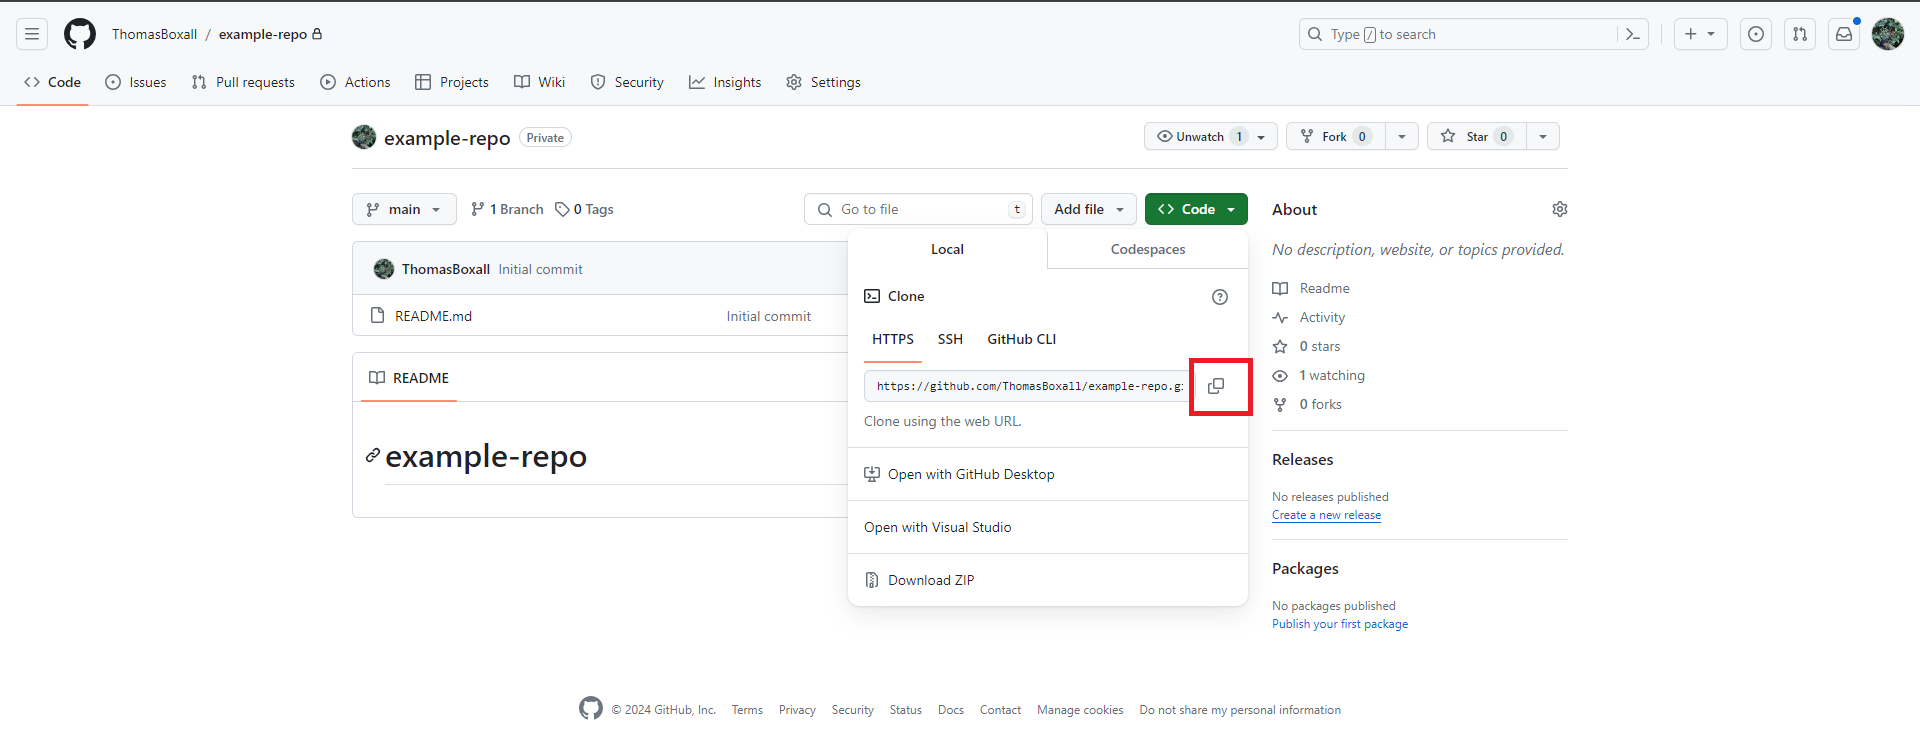
\includegraphics[width=0.9\textwidth]{assets/gitclone.png}
    \caption{Clone options within GitHub web}
\end{figure}

Once you have copied the repository's URL, open your terminal and navigate to the folder in which you wish to clone the repository. I find it easiest to use have a \verb|git| directory within my user folder into which I clone all my repositories.\\

When you are in the suitable folder, clone the repository using the \verb|git clone [url] [folder-to-clone-into]| command. For example, if I wanted to clone my example repository into the folder \verb|example-repo/| I would enter the following:
\begin{verbatim}
    git clone https://github.com/ThomasBoxall/example-repo.git example-repo/
\end{verbatim}

You should get an output which looks something like the following:
\begin{verbatim}
    Cloning into 'example-repo'...
    remote: Enumerating objects: 3, done.
    remote: Counting objects: 100% (3/3), done.
    remote: Total 3 (delta 0), reused 0 (delta 0), pack-reused 0
    Receiving objects: 100% (3/3), done.
\end{verbatim}

You can now navigate into the folder git will have created while cloning.\\

Congratulations! You now have a local copy of the Git Repository on your computer, well done. Go pat yourself on your back! Next up is the fun of branches\dots

\section{Part II: Working With Branches}
When developing, we want to be able to isolate our different development strands into different `boxes'. This is done with \textit{Branch}. In essence, a branch is an offshoot of the current repository, where you can make changes (this could be adding a new feature or fixing a bug), then it can be \textit{merged} back to the main branch. The key thing to remember is that a branch is for a feature, not a person.\\

In this example, I'm going to use a branch to add a few lines of text to the \verb|README.md| of my project. The first thing I will do is get a list of all branches currently on my local machine with the command \verb|git branch|:
\begin{verbatim}
    * main
\end{verbatim}

As you can see above, I only have one branch. I can create a new branch by adding the name of the new branch onto the end of the command we used above:
\begin{verbatim}
    git branch adding-content-to-readme
\end{verbatim}
The above command will not return any text to me. I can now re-run \verb|git branch| to list all my local branches:
\begin{verbatim}
      adding-content-to-readme
    * main
\end{verbatim}
As you can see above, I now have two branches, \verb|main| and \verb|adding-content-to-readme|. My current branch is \verb|main| which can be seen by the asterisk next to it.\\

To change branch to my new branch, I have to use the \verb|checkout| command:
\begin{verbatim}
    git checkout adding-content-to-readme
\end{verbatim}
This will give you an output:
\begin{verbatim}
    Switched to branch 'adding-content-to-readme'
\end{verbatim}

Great, now I can make changes to the local copy of my code and it will stay within my new branch and not effect the \verb|main| branch. Some editors will tell you which branch you are using, for example \textit{VS Code} displays it in the bottom left hand corner of the window.

\section{Part III: Committing Changes}
Once you've finished working on the code, or you have completed the fix / feature, or you have something working - it's time to commit the code. What this is doing is bundling all the changes you have just made into something called a \textit{commit}, these are stored and therefore mean versions of files can be tracked. This is why it's important to commit frequently, not just once at the end of the project!\\

The first step is to \verb|add| all the changed files to the commit. You can examine what these will be using the \verb|git status| command. You will generally need to just add all files to the commit which can be achieved with the following command:
\begin{verbatim}
    git add .
\end{verbatim}
This will not produce an output.\\

The next step is to issue the commit command. This requires the insertion of a message which is stored with the commit. Make this descriptive as it makes life so much easier if you need to trawl back through a project to find a commit where something broke.
\begin{verbatim}
    git commit -m "feat:added content to readme;"
\end{verbatim}
This will result in something like the output below:
\begin{verbatim}
    [adding-content-to-readme 8314c48] feat:added content to readme;
     1 file changed, 3 insertions(+), 1 deletion(-)
\end{verbatim}
Note that it gives the name of the branch on the top line. Check that this is correct! If it is not, you need to un-commit and un-stage those changes:
\begin{verbatim}
    git reset HEAD^
\end{verbatim}

Assuming you are now satisfied that you're committing to the right branch - you're ready to push. Pushing is the process of pushing the changes from your local machine to the remote server (that's GitHub). This is achieved with the command \verb|git push|. However, as we are using a non-main branch, we need to tell git to push to the right place so we use the following command:
\begin{verbatim}
    git push --set-upstream origin adding-content-to-readme
\end{verbatim}
If you don't do this, git will moan at you and tell you to do it. From now on, while working on this branch, you are able to just use \verb|git push| to push content. When you change branch again, you need to use the long command again. You will get an output after running the push command:
\begin{verbatim}
    Enumerating objects: 5, done.
    Counting objects: 100% (5/5), done.
    Delta compression using up to 8 threads
    Compressing objects: 100% (2/2), done.
    Writing objects: 100% (3/3), 338 bytes | 338.00 KiB/s, done.
    Total 3 (delta 0), reused 0 (delta 0), pack-reused 0
    remote:
    remote: Create a pull request for 'adding-content-to-readme' on GitHub by visiting:
    remote:      https://github.com/ThomasBoxall/example-repo/pull/new/adding-content-to-readme
    remote:
    To https://github.com/ThomasBoxall/example-repo.git
    * [new branch]      adding-content-to-readme -> adding-content-to-readme
    branch 'adding-content-to-readme' set up to track 'origin/adding-content-to-readme'.
\end{verbatim}
The length and content of the push message will vary depending on what you are pushing and where-to. As long as it's not screaming about something, you're fine.

\section{Part IV: Merging Branches}
This section is to be completed once you have finished the feature, fixed the bug or done whatever you deemed the branch to be used for. By the end of this section, the branch you have been using will no longer be in existence.\\

We will be using the GitHub web application to merge our branches. It is possible to use the CLI, however this doesn't allow for Pull Requests which are fundamental parts of the code review process.\\

First, navigate to the new branch and GitHub should prompt you to \textit{Compare \& pull request} - this is precisely what we want to do!
\begin{figure}[H]
    \centering
    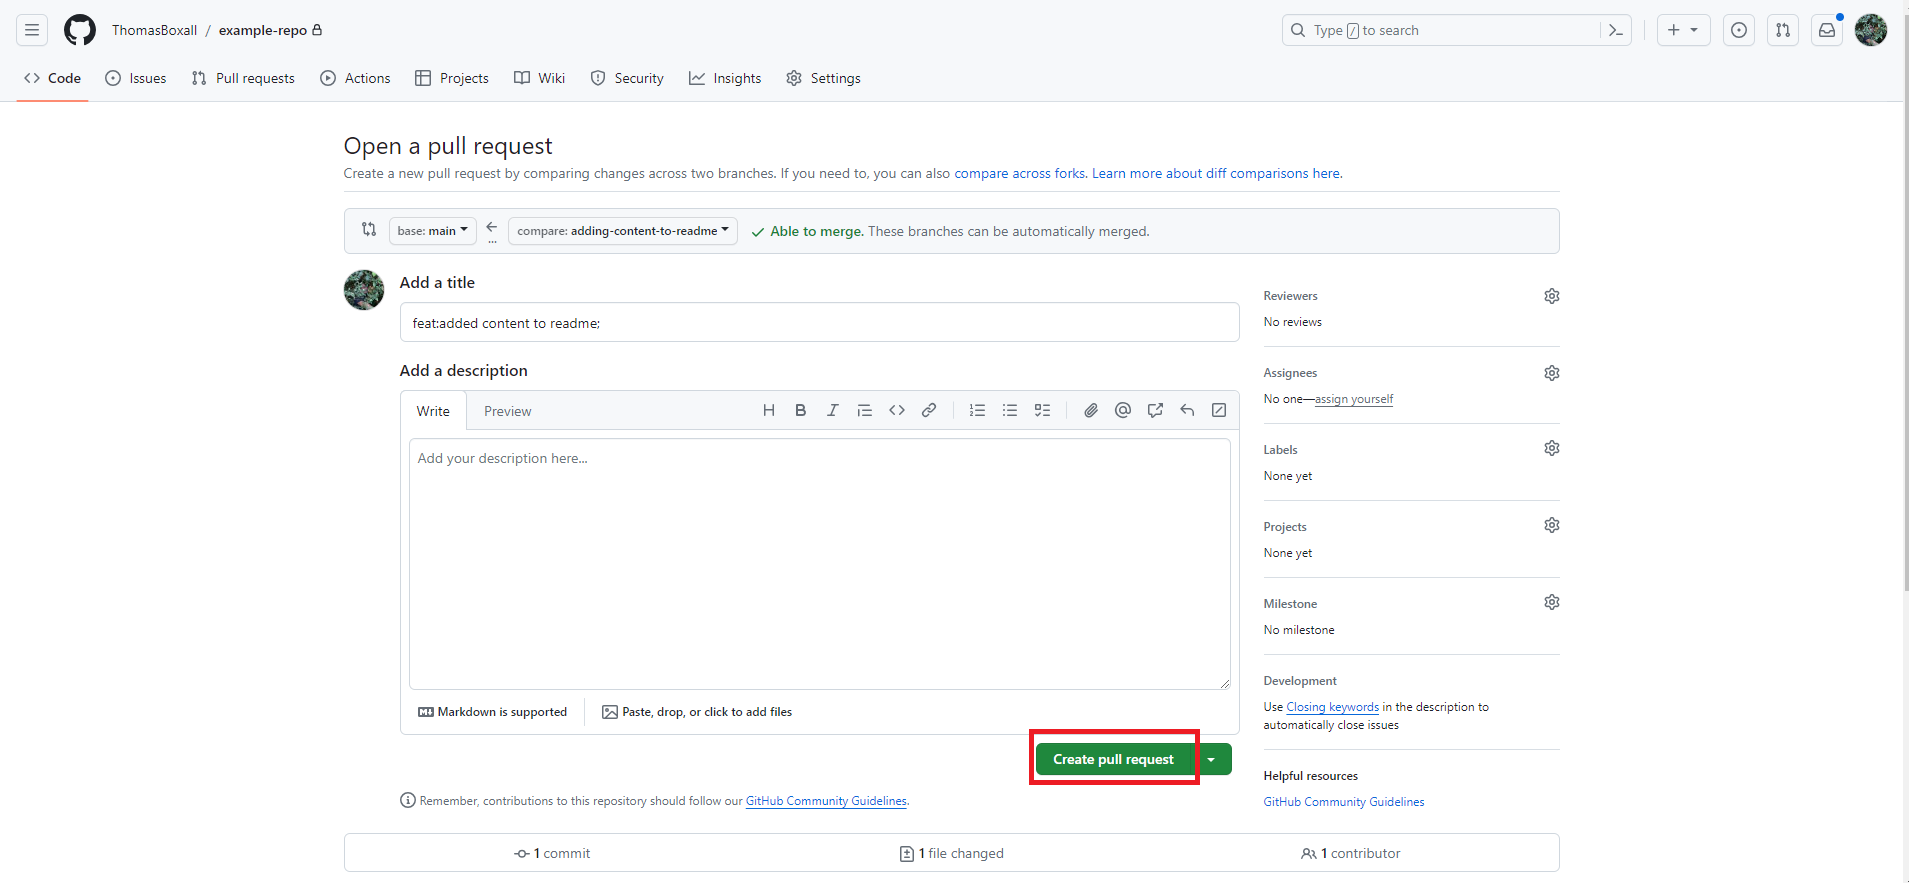
\includegraphics[width=0.9\textwidth]{assets/gh-compare-pr.png}
    \caption{Compare \& pull request page on GitHub}
\end{figure}

Enter any details in the title and description where relevant. If you have a Project Management tool which you are using, it might be advisable to enter something into the description of the PR which references this. If you have a specific person to assign to review the PR, assign them on the right hand side; then press the `Create pull request' button.\\

Someone else will now need to review the Pull Request and `Merge Pull Request' if the PR is accepted. Once the PR is merged, the merger should delete the branch on GitHub as this keeps the repository clean and tidy!
\begin{figure}[H]
    \centering
    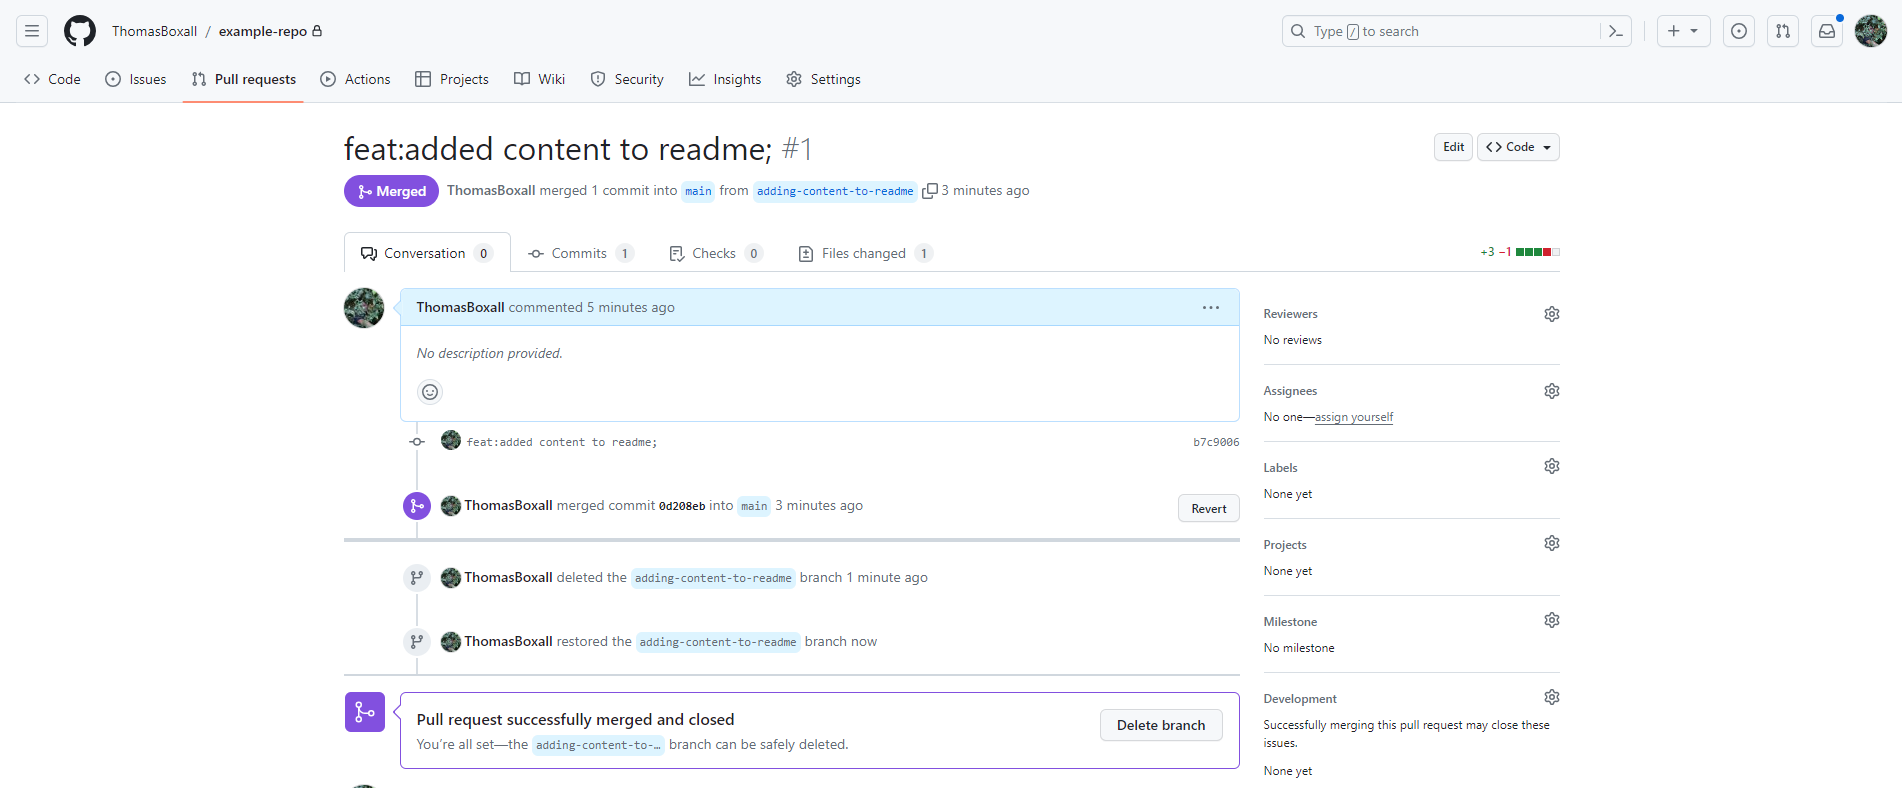
\includegraphics[width=0.9\textwidth]{assets/gh-delete-branch.png}
    \caption{Delete branch prompt on GitHub}
\end{figure}

You will then probably want to delete your local branch. This can be done through the following steps:
\begin{enumerate}
    \item Checkout the main branch
    \begin{verbatim}
        git checkout main
    \end{verbatim}
    which outputs
    \begin{verbatim}
        Switched to branch 'main'
        Your branch is up to date with 'origin/main'.
    \end{verbatim}
    \item Pull the latest version of \verb|main|
    \begin{verbatim}
        git pull
    \end{verbatim}
    which outputs
    \begin{verbatim}
        remote: Enumerating objects: 1, done.
        remote: Counting objects: 100% (1/1), done.
        remote: Total 1 (delta 0), reused 0 (delta 0), pack-reused 0
        Unpacking objects: 100% (1/1), 922 bytes | 230.00 KiB/s, done.
        From https://github.com/ThomasBoxall/example-repo
          1b16a96..0d208eb  main       -> origin/main
        Updating 1b16a96..0d208eb
        Fast-forward
          README.md | 4 +++-
          1 file changed, 3 insertions(+), 1 deletion(-)
    \end{verbatim}
    \item Delete the local branch
    \begin{verbatim}
        git branch -d adding-content-to-readme
    \end{verbatim}
    which outputs
    \begin{verbatim}
        Deleted branch adding-content-to-readme (was b7c9006).
    \end{verbatim}
    \item (Optional) You can then verify that the branch has been deleted using the \verb|git branch| command which outputs the following:
    \begin{verbatim}
        * main
    \end{verbatim}
\end{enumerate}

\section{Other Important Commands}
There are two other important Git commands which you will probably find yourself using quite frequently.
\subsection{Status}
The \verb|git status| command can be used to get the status of your current repository and any changes made against the remote repository. An example output is shown below, where the local repository is up to date with the remote one:
\begin{verbatim}
    On branch main
    Your branch is up to date with 'origin/main'.

    nothing to commit, working tree clean
\end{verbatim}
Another example output is shown below where a change has been made to the local repository that hasn't been committed or pushed yet:
\begin{verbatim}
    On branch main
    Your branch is up to date with 'origin/main'.

    Changes not staged for commit:
    (use "git add/rm <file>..." to update what will be committed)
    (use "git restore <file>..." to discard changes in working directory)
            deleted:    README.md

    no changes added to commit (use "git add" and/or "git commit -a")
\end{verbatim}

\subsection{Pull}
The \verb|git pull| command will `download' the latest changes from the remote repository to the local one on your machine. You must do this every time you sit down to work as otherwise there will be lots of nasty merge conflicts which have to be solved by hand.

\end{document}